\section{Low-dimensional rigidity and curved deformations}
\label{low:section}
\begin{figure}[htbp]
  \centering
  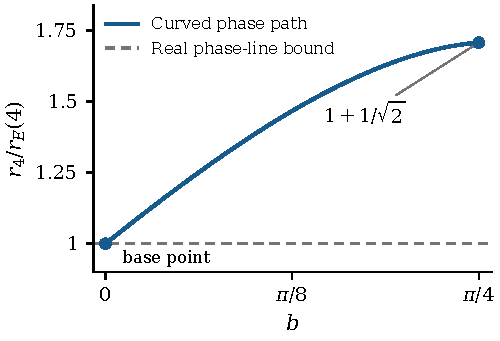
\includegraphics[width=\columnwidth]{figures/fig3_curved.pdf}
  \caption{Enhancement at $n=4$ along the explicit curved phase path.
  The solid curve is $r_4/r_E(4)=\cos[b+\delta(b)]-\sin\delta(b)$, evaluated from the closed-form root on $0\leq b\leq\pi/4$.
  It increases from $1$ to $1+1/\sqrt2$.
  The dashed level is the radius bound for all real phase lines through the specified base point. Plotting code was prepared with OpenAI Codex (GPT-6) assistance and checked against the stated formulas.}
  \label{fig:curved}
\end{figure}


The threshold $n=5$ has a geometric explanation within the fixed
phase representation.  At $n=3$ the specified measurement is locally
isolated.  At $n=4$ the regularity equations admit deformations, but
every admissible phase line fails to increase the radius.  A curved path
through the same point does increase it.

\begin{proposition}[Local rigidity at $n=3$]
\label{low:rigidity}
In the fixed Pauli-orbit representation, the specified EJM at $n=3$ is
isolated in a neighborhood of its phase vector, after removing the overall
phase.
\end{proposition}
Indeed, the seven independent phases give eight differences between signed
local components.  Seven of their derivatives have determinant
$1/4096$ at the specified point.  The inverse function theorem therefore
isolates the zero of these seven equations.  Since every signed component
equals $1/4$ at that point, the squared regularity conditions are equivalent
to signed equality in a neighborhood.  The exact Jacobian in
Appendix~\ref{low:app-rigidity} turns the numerical rank reported in
Ref.~\cite{PauwelsGisin2026} into an analytic local statement.

For $n=4$, write an arbitrary phase line as
\begin{equation}
 M_d(t)=C_4\operatorname{diag}
 \bigl(i^{f_0(z)}e^{itd_z}\bigr)H^{\otimes4},\qquad d_0=0.
 \label{low:line}
\end{equation}
The normalization $d_0=0$ removes only a common phase; the remaining
15 entries of $d$ are arbitrary real numbers.

Figure~\ref{fig:curved} compares the phase-line bound with the curved
enhancement described below.
\begin{theorem}[Phase lines and a curved enhancement at $n=4$]
\label{low:theorem}
Every line~\eqref{low:line} that remains a common-radius regular
tetrahedral measurement in a neighborhood of $t=0$ has
\begin{equation}
 r_d(t)=r_E(4)|\cos(\omega t)|\le r_E(4)
 \label{low:line-bound}
\end{equation}
for some real $\omega$.  Nevertheless, there is an explicit curved phase
path through the same measurement for which
\begin{equation}
 r_4\bigl([0,\pi/4]\bigr)
 =\left[r_E(4),\left(1+\frac1{\sqrt2}\right)r_E(4)\right],
 \label{low:curve-range}
\end{equation}
and the radius is strictly increasing along the path.
\end{theorem}

The obstruction to straight paths is stronger than the Boolean bound.
The full linearized constraint kernel is four dimensional; second-order
conditions eliminate one direction except for a single candidate ratio,
and a nonzero third-order term eliminates that candidate.  The remaining
directions form two planes, each giving only the cosine law
\eqref{low:line-bound}.  Their explicit classification is given in
Appendix~\ref{low:app-lines}.

To construct a path that can leave these planes, allow two independent
real parameters $b,\delta$ and set $\theta_z=bu_z+\delta v_z$, using the
two fixed integer masks $u,v$ in Eq.~\eqref{low:masks}.
For these phases, the signed physical Pauli components of the seed take
only two values: ten components equal $T/8$, whereas the components of
$X_1$ and $-Y_4$ equal $H/8$, where
\begin{align}
 T&=\cos(b+\delta)-\sin\delta,\nonumber\\
 H&=\cos b+2\sin\delta\cos b+4\sin b\cos b.
 \label{low:two-components}
\end{align}
These identities hold before a path is selected.  The signed regularity
condition is therefore $H=T$, a quadratic equation in $\tan(\delta/2)$.

The root branch through $(b,\delta)=(0,0)$ has the following closed
expression.  For $0\le b\le\pi/4$, define
\begin{align}
 A(b)&=\cos b(1+2\sin b),\nonumber\\
 B(b)&=2\cos b+\sin b+1,\qquad
 C(b)=2\sin b\cos b,\nonumber\\
 \delta(b)&=-2\arctan\frac{2C(b)}
 {B(b)+\sqrt{B(b)^2-4A(b)C(b)}}.
 \label{low:delta}
\end{align}
With this choice, the phase path and measurement are
\begin{equation}
 \begin{aligned}
 \theta_z(b)&=bu_z+\delta(b)v_z,\\
 M_4(b)&=C_4\operatorname{diag}
 \bigl(i^{f_0(z)}e^{i\theta_z(b)}\bigr)H^{\otimes4}.
 \end{aligned}
 \label{low:curve}
\end{equation}
Thus all signed components coincide on the entire explicit path.
Unitarity and the Pauli-orbit relation then give the complete measurement
and its fixed local tetrahedra.  Its common radius is
\begin{equation}
 r_4(b)=r_E(4)\bigl[\cos\bigl(b+\delta(b)\bigr)-\sin\delta(b)\bigr].
 \label{low:curve-radius}
\end{equation}
The radicand and denominator in Eq.~\eqref{low:delta} are strictly
positive on the closed interval $0\le b\le\pi/4$.
Appendix~\ref{low:app-curve} proves that the branch is well defined and
that its radius is strictly increasing throughout this interval.
Both angles vanish at $b=0$, so the original measurement is recovered
column by column.  At the other endpoint $\delta(\pi/4)=-\pi/4$, giving
the upper endpoint in Eq.~\eqref{low:curve-range}.
The curved path leaves the two planes of admissible line directions and
has $r'_4(0)=\sqrt3/6>0$.

The larger value $3r_E(4)$ already occurs at a different measurement at $n=4$ in Ref.~\cite{PauwelsGisin2026}.  The purpose of
Eq.~\eqref{low:curve} is to increase the radius through the specified
$f_0$ measurement and explain the required curvature.  The parameter
segment of that earlier family contains no measurement equivalent to
this specified point under local unitaries, qubit permutations, and
outcome relabeling.  Appendix~\ref{low:app-invariant} gives a short
certificate using the one-qubit spectrum and the sum of the three
$2|2$ purities.  Whether a larger regular-tetrahedral solution manifold
connects the two families remains open.
